\section{XF Core}
\subsection{Événements}
La classe XFEvent est composée d'un id d'événement, et d'un type d'événement :
\begin{figure}[H]
    \centering
    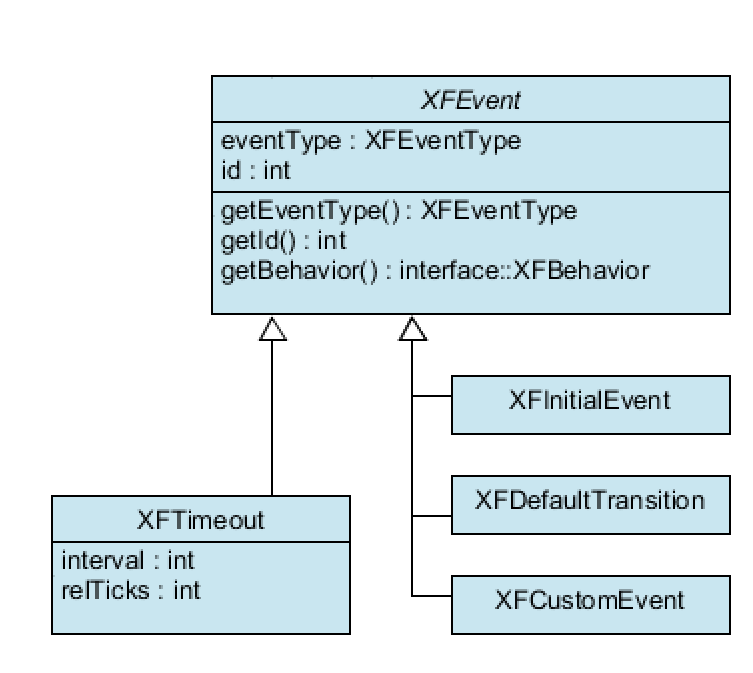
\includegraphics[width=0.5\textwidth]{Images/xf/xfevent.PNG}
    \caption[Diagramme de classe du XFEvent]{Diagramme de classe du XFEvent (provenant du diagramme
        de classe XF de la documentation \emph{Simplified XF}\footnotemark[1])}
\end{figure}
\footnotetext[1]{\cite{documentation}}
Les classes XFInitialEvent, XFDefaultTransition sont simplement des événements avec un type
fixe. La classe XFCustomEvent est un alias de XFEvent. Finalement, la classe XFTimeout ajoute
deux choses : une intervalle et un nombre de tick restant. En effet, le timeout est une
sorte de minuterie générant un événement une fois le temps écoulé. Cette gestion des timeout
sera détaillée dans la partie \emph{"Timeout Manager"}\newpage

\subsection{Machines d'états}
La classe XFBehavior sert de base pour créer des machines d'états. Elle possède un lien
vers le Dispatcher et a toujours un événement courant sauvegardé.
\begin{figure}[H]
    \centering
    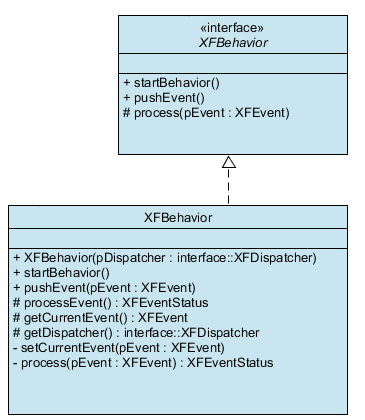
\includegraphics[width=0.5\textwidth]{Images/xf/XFBehavior.PNG}
    \caption[Diagramme de classe du XFBehavior]{Diagramme de classe du XFBehavior
    (provenant du diagramme de classe XF de la documentation
    \emph{Simplified XF}\footnotemark[1])}
\end{figure}
\footnotetext[1]{\cite{documentation}}
L'utilisation d'une interface est utile pour implémenter des machines d'états personnalisées
en héritant de XFBehavior. L'interface permet un polymorphisme flexible et optimal.\newpage

\subsection{Interfaces}
Le cœur n'a pas de lien direct sur les ports du XF, car ceci peuvent être modifié d'un
système à l'autre. Pour faire en sorte que le cœur n'est jamais besoin de modification,
il accède aux ports via des interfaces.
\begin{figure}[H]
    \centering
    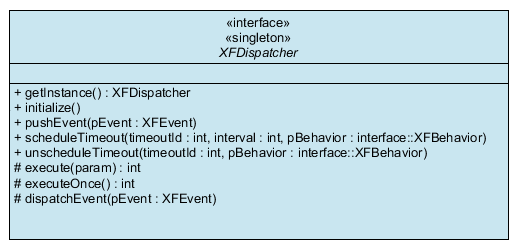
\includegraphics[width=0.6\textwidth]{Images/xf/XFDispatcherInterface.PNG}
    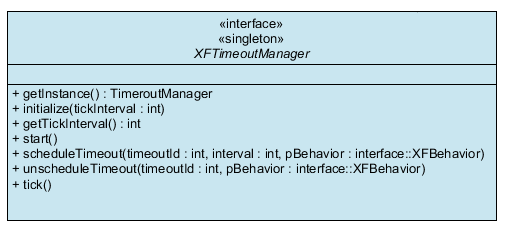
\includegraphics[width=0.6\textwidth]{Images/xf/XFTimeoutManagerInterface.PNG}
    \caption[Diagramme de classe des interfaces des ports]{Diagramme de classe des
    interfaces des ports(provenant du diagramme de classe XF
    de la documentation \emph{Simplified XF}\footnotemark[1])}
\end{figure}
\footnotetext[1]{\cite{documentation}}
Ces interfaces sont celles du XFDispatcher et du XFTimeoutManager. Aucun autre port 
n'est accessible depuis le cœur. \newpage

\section{XF Port}
Tous les ports du XF se présente ainsi :
\begin{figure}[H]
    \centering
    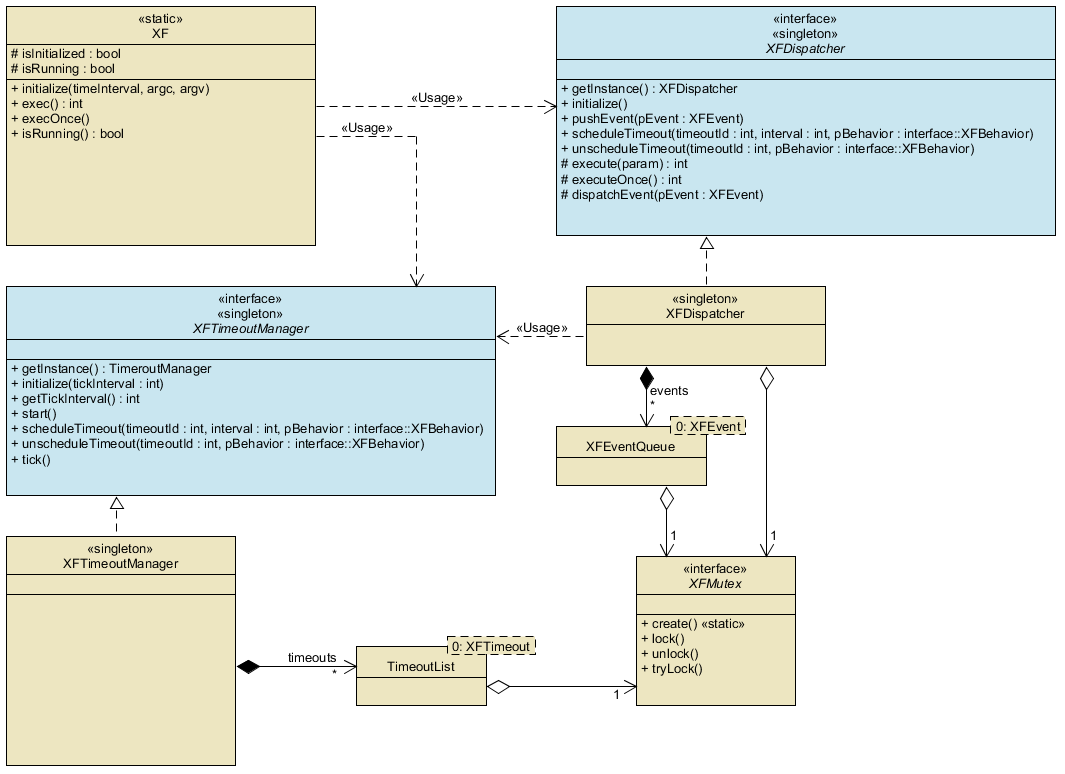
\includegraphics[width=\textwidth]{Images/xf/XFPorts.PNG}
    \caption[Diagramme de classe des ports]{Diagramme de classe des ports
    (provenant du digramme de classe XF de la documentation \emph{Simplified XF}\footnotemark[1])}
\end{figure}
\footnotetext[1]{\cite{documentation}}

\subsection{XF}
Cette classe présente simplement la tâche "XF", elle indique si le XF est en cours d'utilisation
et possède deux méthodes :
\begin{itemize}
    \item exec() -> Tourne dans une boucle infinie appelant le Dispatcher
    \item execOnce() -> Plus adaptée aux systèmes embarqués, doit être appelée dans la boucle
            infinie du programme
\end{itemize}

\subsection{Dispatcher}
Le Dispatcher s'occupe d'une queue d'événements. Il peut recevoir des événements de 2 endroits : Le timeout manager, qui renvoie les timeouts échus, et des machines
d'états directement.
Son rôle est d'ensuite dispatché les événements dès que possible, dans l'ordre :
premier arrivé, premier servi (comme une file d'attente).

\subsection{Timeout Manager}
Le Timeout Manager utilise un timer du système (QTimer sur PC,
timer d'interruption sur système embarqué) pour décrémenter tous nos
Timeouts (les fameuses minuteries).
Une implémentation bête et simple serait d'avoir une table de tous les timeouts
et de décrémenter les ticks restants à chaque "tick" de notre timer.
Cependant, une telle implémentation, bien que très simple, pause un gros problèmes lorsqu'il
y aura énormément de timeout. En effet, le fait de décrémenter les ticks de chaque timeout, un à
un prends rapidement du temps, ce qui ralenti l'exécution et casse le principe temps réel de ce
XF.\\
La solution plus intelligente serait de placer les timeouts dans l'ordre, et de ne décrémenter
que le premier timeout :
\begin{figure}[H]
    \centering
    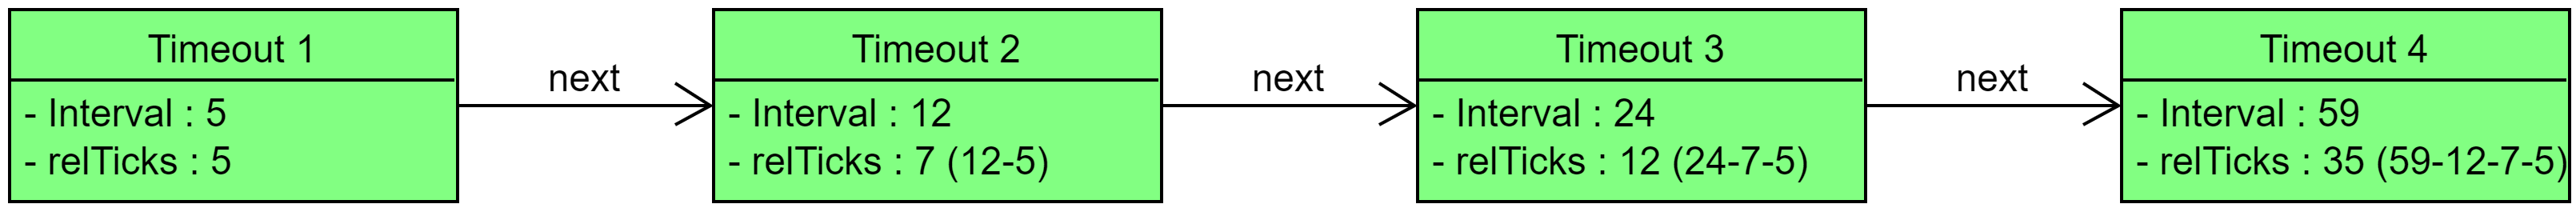
\includegraphics[width=0.85\textwidth]{Images/xf/timeoutList.PNG}
    \caption[A sorted timeout queue]{Exemple de queue de timeout triée}
\end{figure}
Ainsi, quand le premier timeout sera échu, il restera 7 ticks au second, et ainsi de suite.
Il faut donc un algorithme de placement intelligent :
\begin{figure}[H]
    \centering
    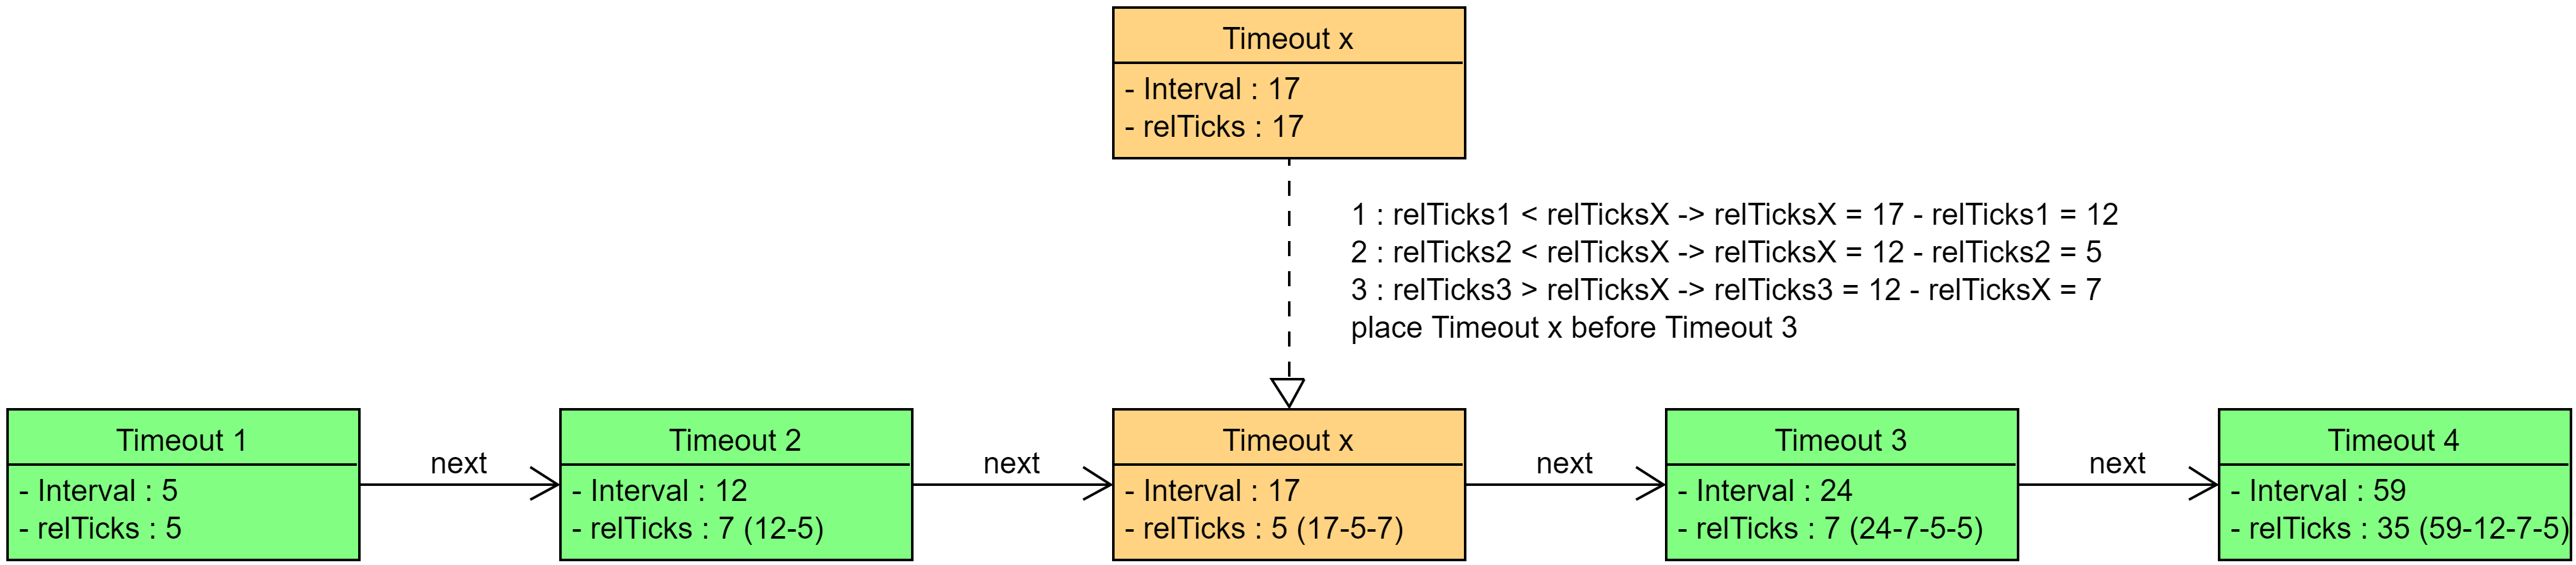
\includegraphics[width=\textwidth]{Images/xf/timeoutSmartList.png}
    \caption{Plaçage intelligent de nouveau timeout}
\end{figure}
L'algorithme procède ainsi : il compare le nouveau timeout au premier de la liste,
si le ticks restants du nouveau sont plus petits que ceux du premier, on le place 
ici et on retire des ticks restants au premier. Sinon, on passe au prochain timeout
de la liste, on retire les ticks restants du premier sur notre nouveau timeout et on continue l'opération jusqu'à la fin.
Si le timeout n'a pas trouvé sa place au milieu des autres, on le place simplement à
la fin, et ses ticks restants seront déjà corrects.\\
À chaque fois qu'un timeout est échu, il n'est pas supprimé, mais directement 
transmis au Dispatcher. Étant donné que timeout hérite de XFEvent, il peut donc
être gérer comme un événement classique.

\subsection{Mutex}
Le Mutex est un mécanisme, dit d'Exclusion Mutuelle (MUTual EXclusion), qui
permet de ne donner l'accès à un objet qu'à un seul thread à la fois.

\emph{Imaginons une salle avec beaucoup de monde qui argumente en même temps, personne
ne se comprends. Maintenant, ajoutons un modérateur et 
un canard en plastique donnant le droit de parole. 
Si vous n'avez pas le canard en plastique, vous n'avez pas le droit de parler,
vous pouvez seulement lever la main pour indiquer que vous voulez parler.
Une fois que la personne en possession du canard en plastique a fini de parler,
elle doit rendre le canard en plastique au modérateur,
qui le transmettra au prochain.}\\
\emph{On remplace canard en plastique par Mutex, et personne par thread, et le fonctionnement est le même.} \footcite{mutex}